\documentclass{reportClass}

\title{Torque in a Variable Reluctance Machine}
\author{G\"{o}ksenin Hande Bayazıt}
%\date{January 2019}
\universityName{Middle East Technical University}
\departmentName{Department of Electrical and Electronics Engineering}
\className{EE568 - Selected Topics on Electrical Machines}
\reportName{Project \#1 Report}

\begin{document}
\printtitle

%\tableofcontents

%\newpage

\section{Introduction}

In this project, a simple variable reluctance motor is analyzed using analytical and numerical techniques. Analytical formulations and their results, which are obtained in MATLAB environment, are compared with finite element analysis (FEA) results. The effects and precision of assumptions made for analytical formulations are compared with non-ideal findings. Furthermore, the effects of linear, non-linear material choices, 2D and 3D modelling differences are discussed.\\

All of the models built for analysis of the machine, the results and figures are present in GitHub, and are accessible \href{http://www.github.com/ghandeb/EE568}{in this link}.
 
 
\section{Analytical Calculations}

\par Analytical reluctance modelling of the given electromechanical system requires several assumptions on the system. Some of these assumptions can be listed as follows:

\begin{itemize}
\item Stator and rotor are assumed to be infinitely permeable.
\item Fringing effects are neglected.
\item Leakage flux is ignored.
\item Even $\vec{B}$ distribution is assumed in the core.
\item Non-linear effects have been neglected (Core has already been defined as infinitely permeable material.).
\item Rotor shape is simplified and straight parts between salient and cylindrical parts are ignored.

\end{itemize} 


Saliency of the rotor causes a change in the reluctance as the rotor rotates. Therefore, reluctance and inductance should be modelled as a function of the rotation angle, let's say $\theta$.\\

\begin{figure}[h!]
\centering
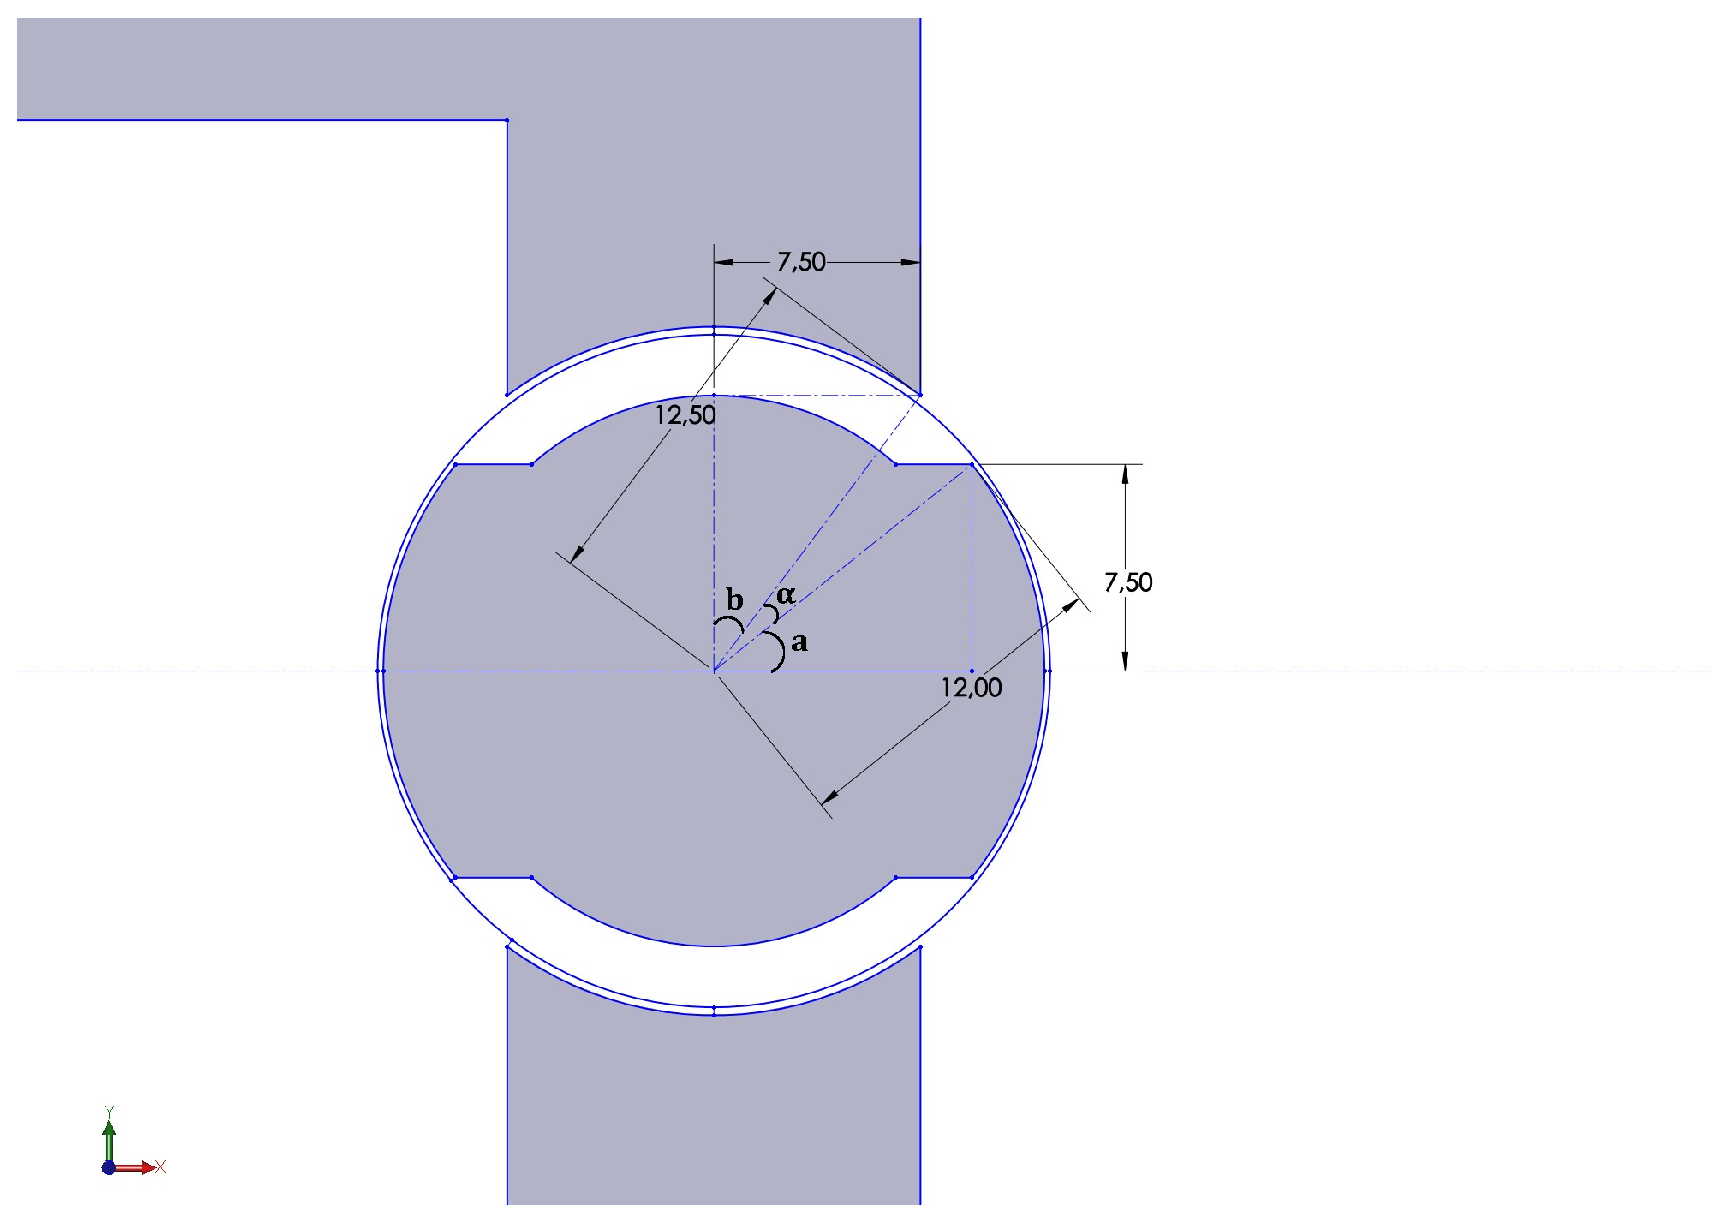
\includegraphics[trim = 40 40 140 60, clip, width=0.6\linewidth]{angles.eps}
\caption{Critical angles of the geometry for accurate reluctance modelling}
\label{fig:angles}
\end{figure}

In Figure \ref{fig:angles}, some critical angles have been defined. For reluctance calculation, $\alpha$ is a critical angle and can be found using trigonometric relations shown in Figure \ref{fig:angles}. As the rotor is in horizontally aligned position ($\theta = 0^\circ$), the air-gap is 2.5 mm. As a result, the system reluctance is maximum and the inductance is at its minimum value. When the rotation angle is $\alpha$, the air-gap becomes 0.5 mm and the reluctance starts to decrease as a function of the surface area of the salient part of the rotor, until the rotation angle becomes $\frac{\pi}{2} - \alpha$. Similarly, between $\frac{\pi}{2} + \alpha$ and $\pi - \alpha$, the reluctance increases as a function of the surface area of the salient part of the rotor.\\

Resultant reluctance formula can be obtained as follows, with respect to the rotation angle,~$\theta$:


$$
\mathcal{R}(\theta) = \left\{
		{\Large
        \begin{array}{ll}
            \frac{2\,g_2}{\mu_0\,2b\,r_0\,\ell} & 0 \leq \theta < \alpha \\ [1em]
            \frac{2\,g_1}{\mu_0\,(\theta - \alpha)\,r_1\,\ell} & \alpha \leq \theta < \frac{\pi}{2} \\ [1em]
            \frac{2\,g_1}{\mu_0\,(\pi - \alpha - \theta)\,r_1\,\ell} & \frac{\pi}{2} \leq \theta < (\pi - \alpha) \\ [1em]
            \frac{2\,g_2}{\mu_0\,2b\,r_0\,\ell} & (\pi - \alpha) \leq \theta \leq \pi
        \end{array} }
    \right.
$$

where $g_1$ is 0.5 mm, $g_2$ is 2.5 mm, $\ell$ is axial length 30 mm, $r_0$ is 12 mm and $r_1$ is 10 mm.\\

Inductance can be defined as:

$$
L(\theta) = \frac{N^2}{\mathcal{R}(\theta)}
$$

Therefore, inductance of the system can be found as a function of $\theta$, accordingly. The change in inductance with respect to $\theta$ is given in Fig. \ref{fig:ind_an}. It can be seen that minimum inductance value is 5\~mH and maximum inductance is 25 \~mH. There will be slight differences both in the waveform and the bounds, because of geometrical approximations and the effect of leakage and fringing flux.\\


\begin{figure}[h!]
\centering
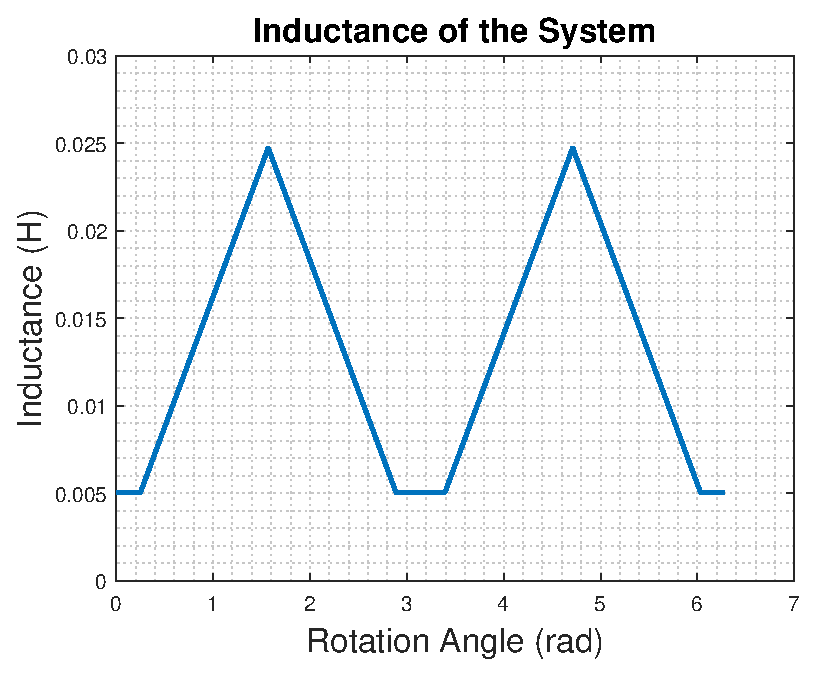
\includegraphics[width=0.6\linewidth]{inductance_analytical.eps}
\caption{Analytical inductance calculation of the system}
\label{fig:ind_an}
\end{figure}


Torque created in the rotor can be calculated by simply taking the derivative of magnetic co-energy with respect to $\theta$. As the system is assumed to be linear, magnetic energy is equal to magnetic co-energy. Therefore, the torque of the rotor can be derived as:

$$
T(\theta) = \frac{1}{2}\,I^2\,\frac{d\,L(\theta)}{d\theta}
$$

With this calculation, torque can be derived as in Fig. \ref{fig:torque_an}. In the real system, inductance transitions are not sharp as in Fig. \ref{fig:ind_an}. As a result, transitions in the torque waveform are expected to be smoother than in Fig. \ref{fig:torque_an}.

\begin{figure}[h!]
\centering
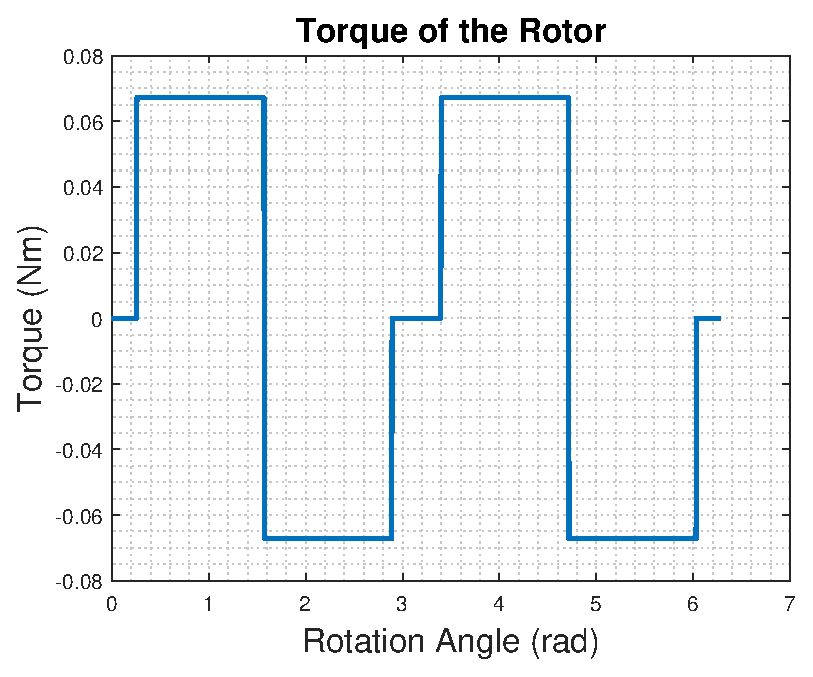
\includegraphics[width=0.6\linewidth]{torque_analytical.eps}
\caption{Analytical torque calculation of the system}
\label{fig:torque_an}
\end{figure}



\section{FE Modelling (2D, Linear Material Properties)}

The geometry is modelled in Ansys Maxwell 2D, using linear material properties with a relative permeability of $\mu_r = 5000$. In Fig. \ref{fig:bvec_lin}, flux density vectors in the system for three different positions of the rotor (0, 45 and 90 degrees) are given. As the rotor is aligned vertically, flux density in the core increases. Furthermore, fringing and leakage flux are also seen in the results in Fig. \ref{fig:bvec_lin}. 

\begin{figure}[h!]
    \centering
  \subfloat[$\theta = 0^\circ$\label{1a}]{%
       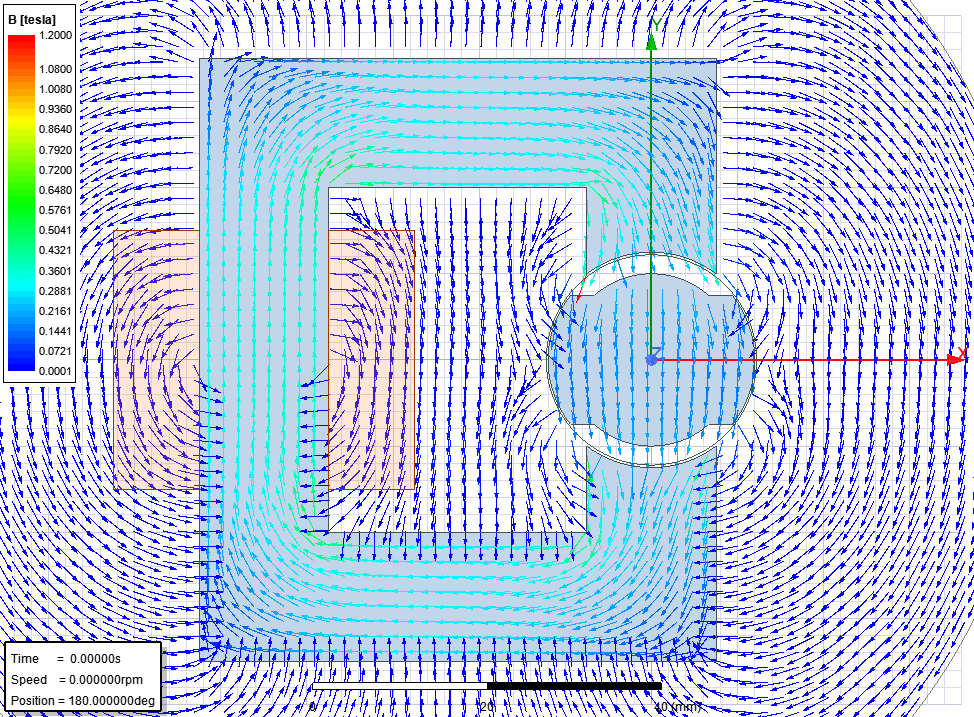
\includegraphics[width=0.3\linewidth]{linear_bvec_0deg.png}}
       \hspace{0.5cm}
  \subfloat[$\theta = 45^\circ$\label{1b}]{%
        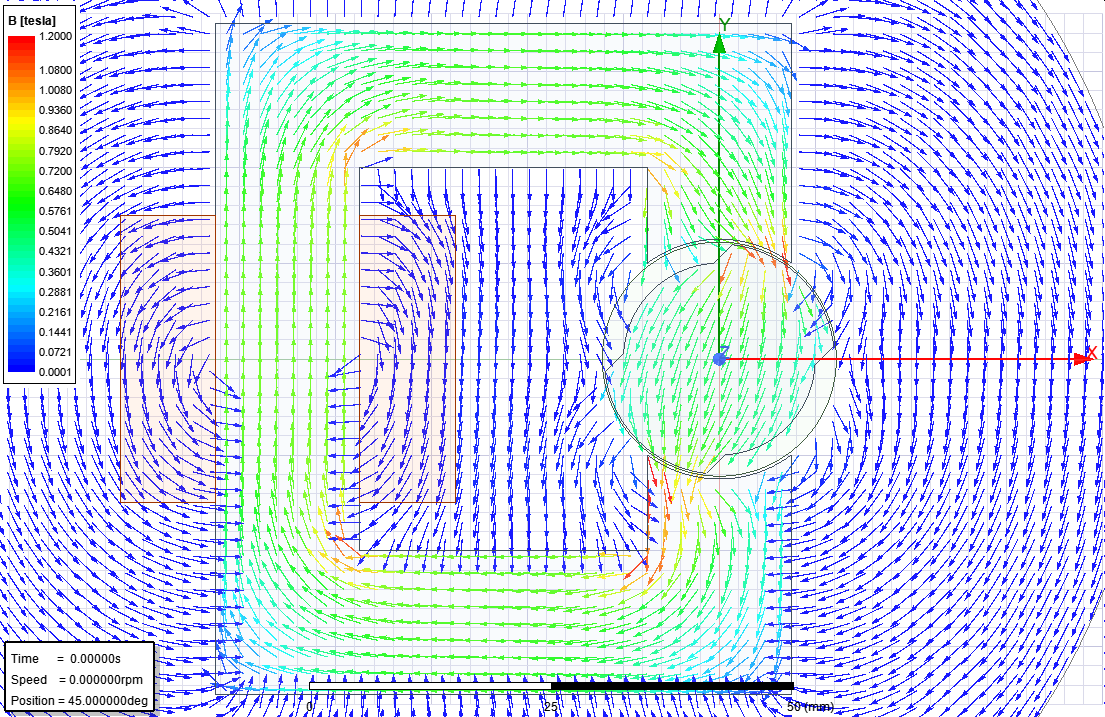
\includegraphics[width=0.3\linewidth]{linear_bvec_45deg.png}}
         \hspace{0.5cm}
  \subfloat[$\theta = 90^\circ$\label{1c}]{%
        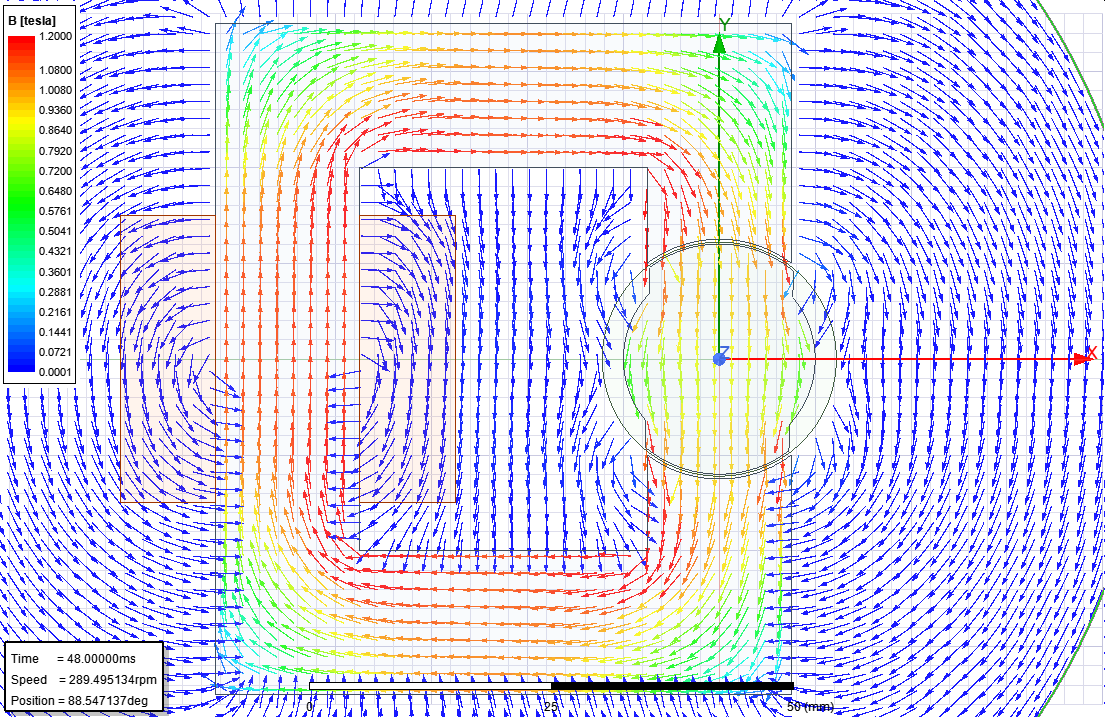
\includegraphics[width=0.3\linewidth]{linear_bvec_90deg.png}}
  \caption{Flux density distribution in the motor for three different positions of the rotor}
  \label{fig:bvec_lin} 
\end{figure}

Inductance of the system is also calculated in Maxwell 2D. \textbf{The initial angle definition of the rotor is equivalent to $\theta = 90^\circ$.} Therefore, the waveform, given in Fig. \ref{fig:ind_lin}, is 90 degrees shifted compared to analytical solution.\\

It is observed that maximum and minimum values of inductance is slightly different than analytical calculation results. The main reason for that is finite permeability of the core material and fringing, leakage flux effects.

\begin{figure}[h!]
    \centering
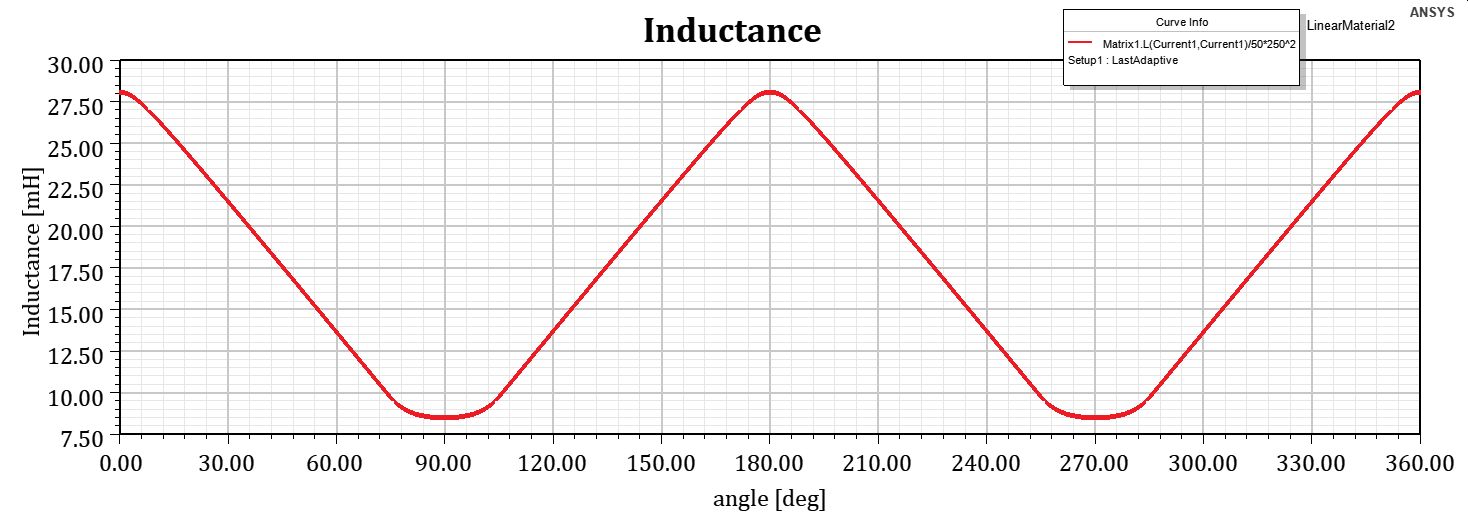
\includegraphics[width=0.75\linewidth]{ind_lin_wrtangle.png}
\caption{Inductance of the system assuming linear material, as a function of rotor angle}
  \label{fig:ind_lin} 
\end{figure}

Torque of the rotor is also obtained as a function of rotor angle and given in Fig. \ref{fig:torque_angle}. The results are compatible with analytical solution results.

\begin{figure}[h!]
\centering
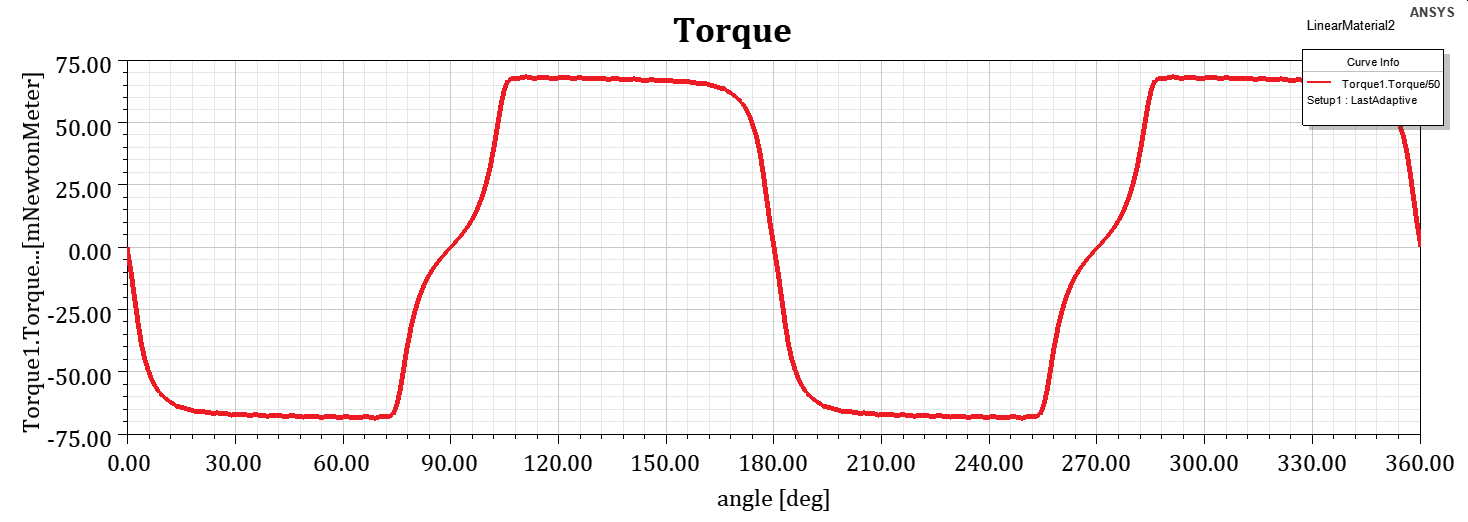
\includegraphics[width=0.75\linewidth]{torque_lin_wrtangle.png}
\caption{Torque of the rotor assuming linear material, as a function of rotor angle}
\label{fig:torque_angle}
\end{figure}

If we rotate the rotor between $45^\circ$ and $-45^\circ$, the torque becomes as in Fig. \ref{fig:torque_time}, as a function of time. A continuous oscillation is observed, as there is no damping or friction in the system.


\begin{figure}[h!]
\centering
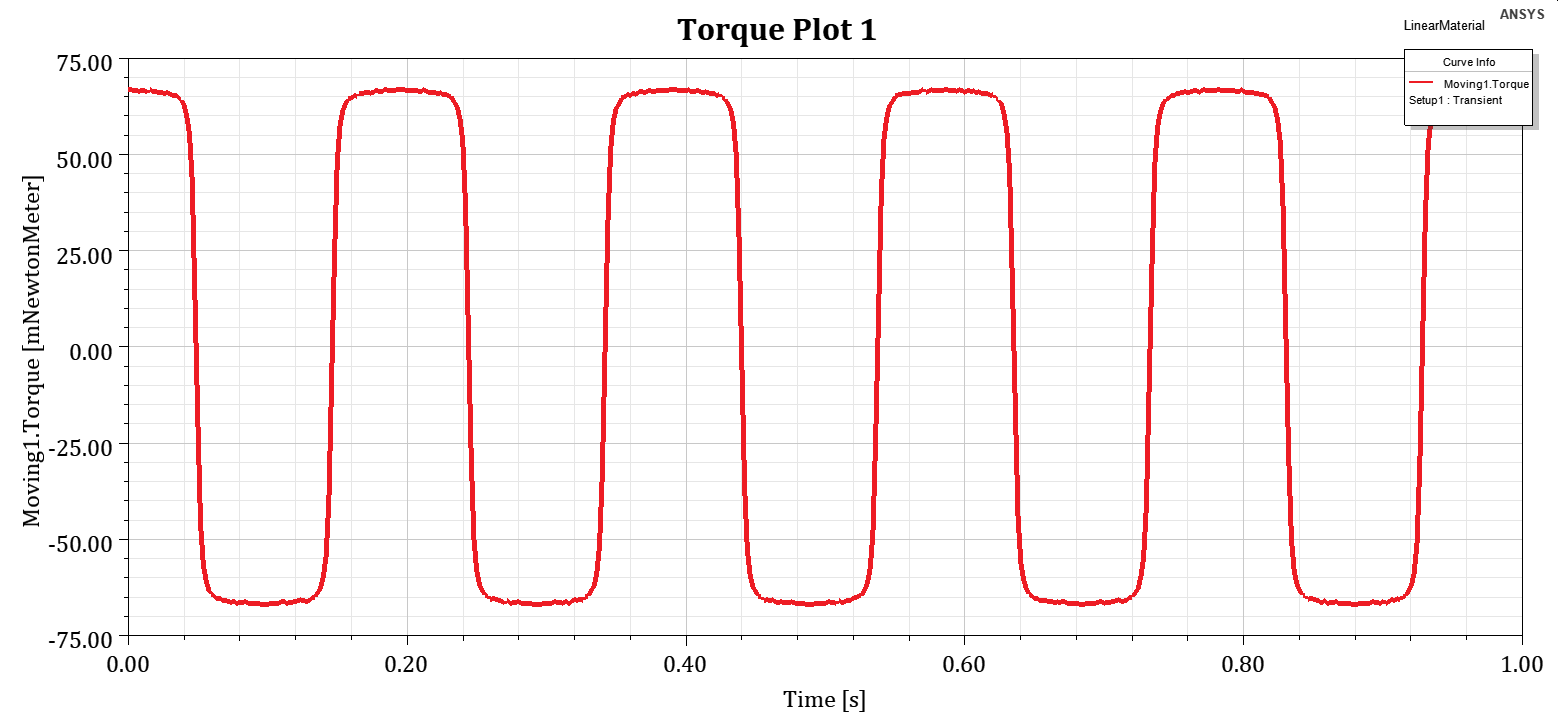
\includegraphics[width=0.75\linewidth]{linear_torque.png}
\caption{Torque of the rotor assuming linear material, as a function of time}
\label{fig:torque_time}
\end{figure}

Magnetic stored energy in the system is obtained using transient analysis. In Fig. \ref{energylin1a}, the energy is calculated when $\theta = 0^\circ$, where in Fig. \ref{energylin1b}, the energy is calculated for $45^\circ < \theta < 135^\circ$. The minimum energy points are when the rotor is horizontally aligned, and is 38~mJ. Stored energy in the system deviates between 38~mJ and 126~mJ.\\

To observe the effects of linear material assumption, energy calculation is compared with the calculation of $\frac{1}{2}\,L\,I^2$. In Fig. \ref{energylin1b}, it can be seen that they are identical.\\


\begin{figure}[h!]
    \centering
  \subfloat[$\theta = 0^\circ$\label{energylin1a}]{%
       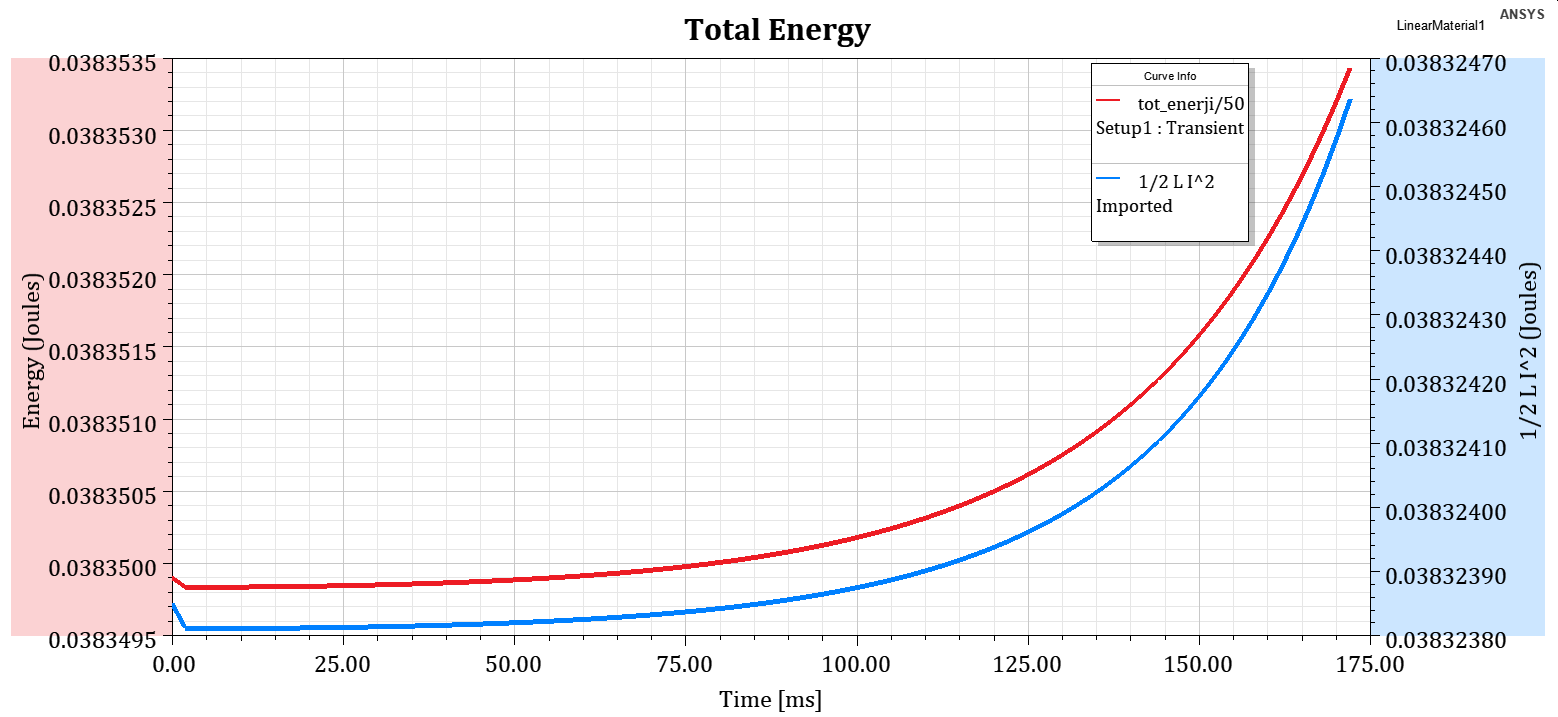
\includegraphics[width=0.45\linewidth]{energy_linear_at0deg.png}}
       \hspace{0.5cm}
  \subfloat[$45^\circ < \theta < 135^\circ$\label{energylin1b}]{%
        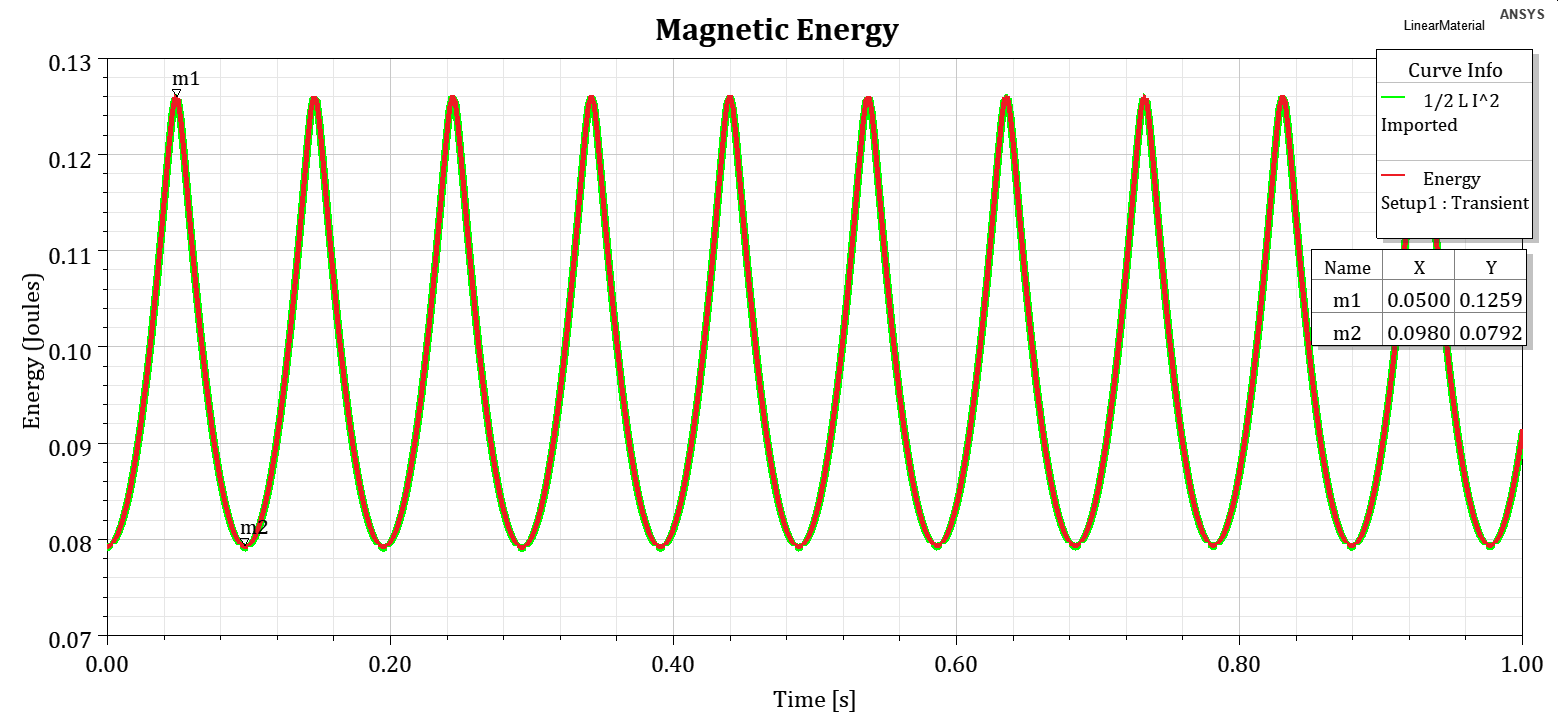
\includegraphics[width=0.45\linewidth]{energy_linear.png}}

  \caption{Magnetic stored energy in the system, assuming linear material properties}
  \label{fig:energy_lin} 
\end{figure}



\section{FE Modelling (2D, Non-linear Material Properties)}


The geometry is modelled in Ansys Maxwell 2D, also using non-linear material properties with a BH curve given in Fig.\ref{fig:bh}. In Fig. \ref{fig:bvec_nonlin}, flux density vectors in the system for three different positions of the rotor (0, 45 and 90 degrees) are given. As the rotor is aligned vertically, flux density in the core increases. Compared to the results obtained assuming linear material, the saturation of the material is observed when the rotor is vertically aligned.\\

\begin{figure}[h!]
\centering
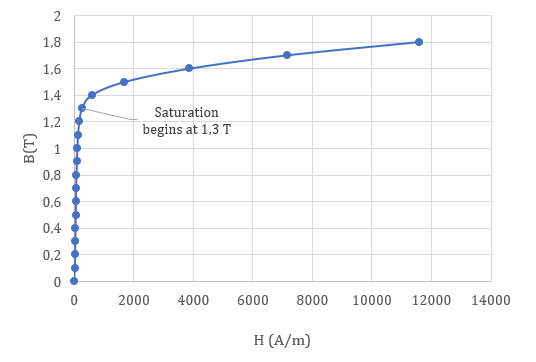
\includegraphics[width=0.6\linewidth]{bh_curve_m270_35a.png}
\caption{BH curve of M270-35A steel}
\label{fig:bh}
\end{figure}


\begin{figure}[h!]
    \centering
  \subfloat[$\theta = 0^\circ$\label{1a}]{%
       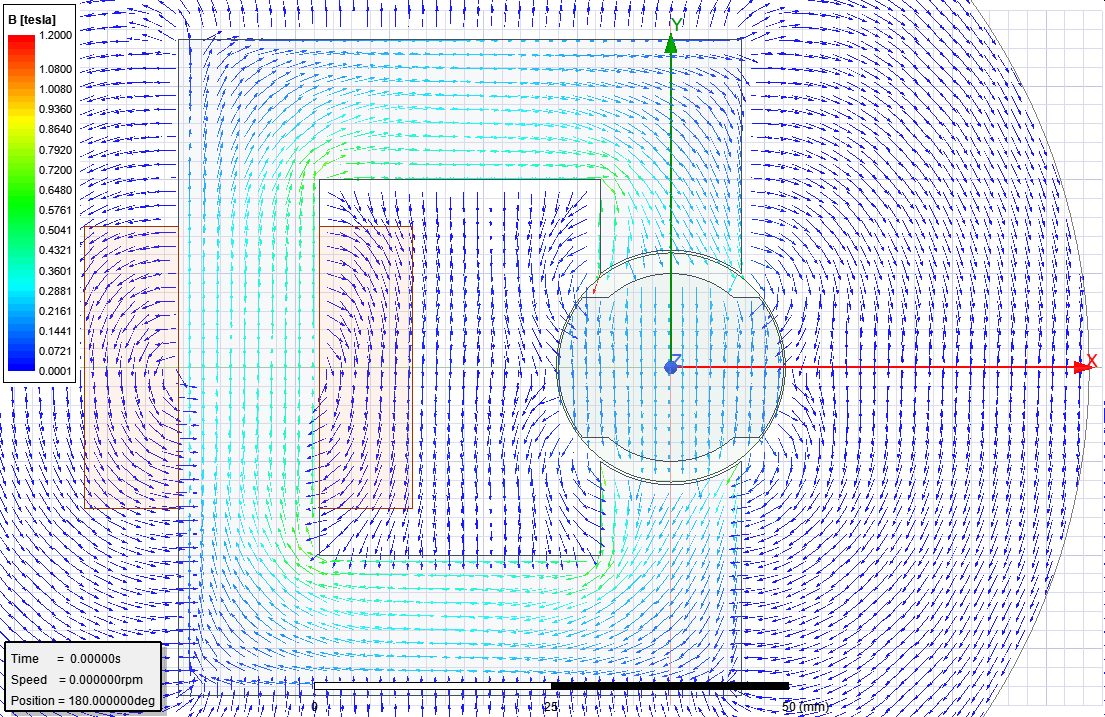
\includegraphics[width=0.3\linewidth]{nonlinear_bvec_0deg.png}}
       \hspace{0.5cm}
  \subfloat[$\theta = 45^\circ$\label{1b}]{%
        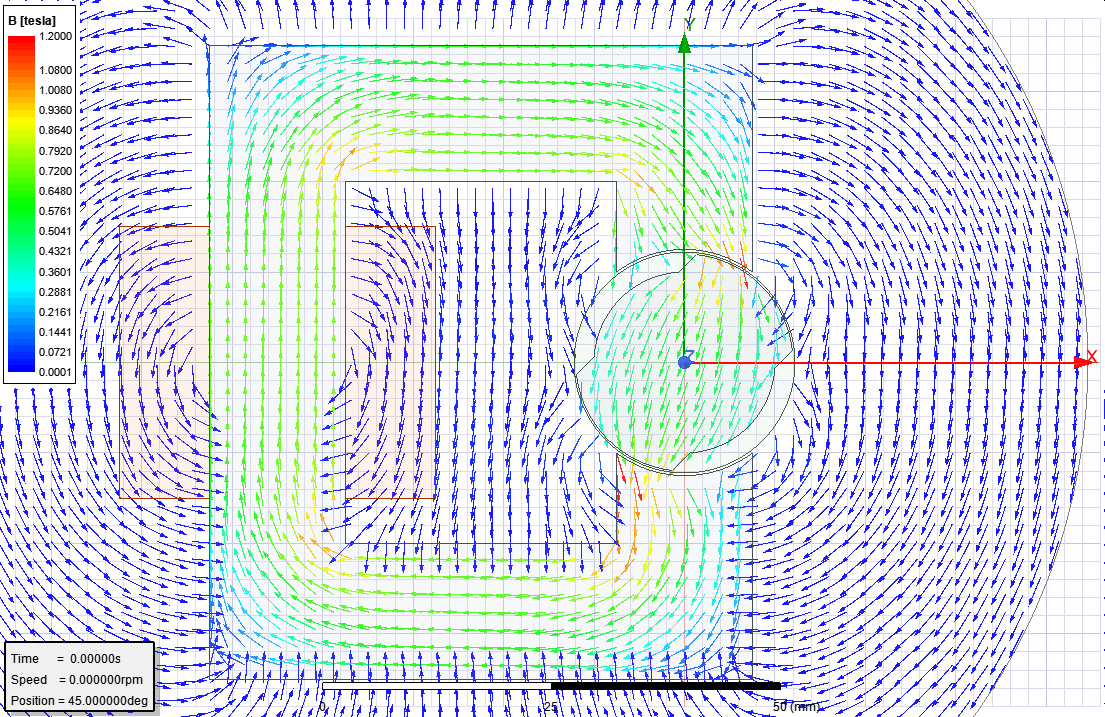
\includegraphics[width=0.3\linewidth]{nonlinear_bvec_45deg.png}}
         \hspace{0.5cm}
  \subfloat[$\theta = 90^\circ$\label{1c}]{%
        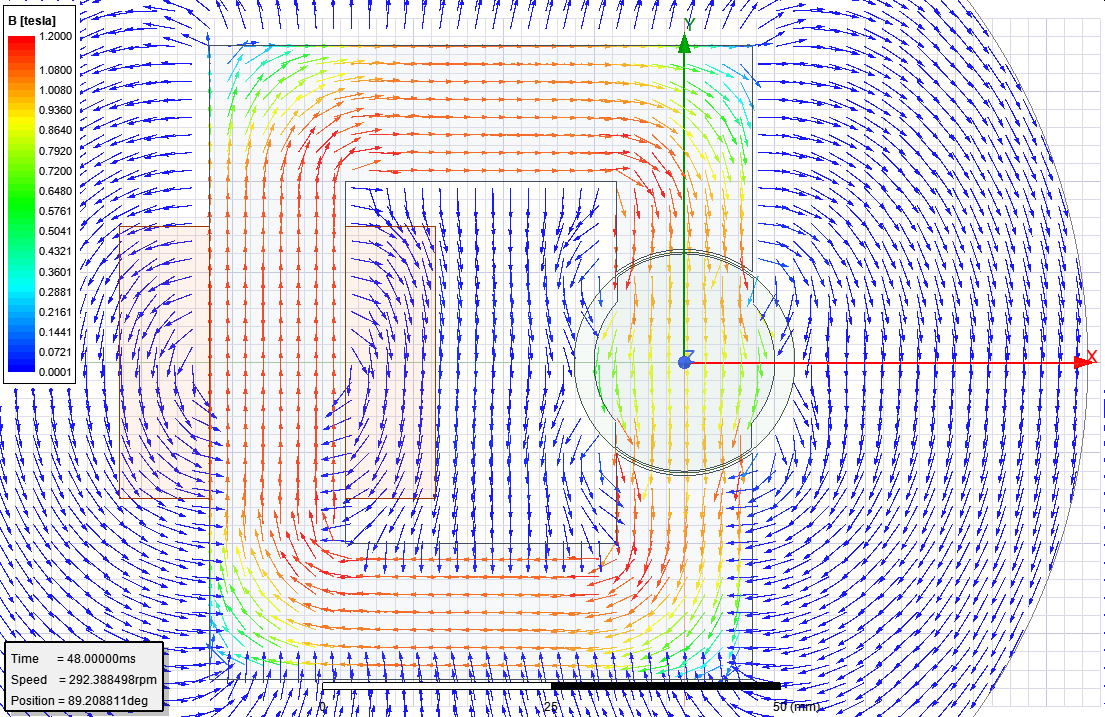
\includegraphics[width=0.3\linewidth]{nonlinear_bvec_90deg.png}}
  \caption{Flux density distribution in the motor for three different positions of the rotor}
  \label{fig:bvec_nonlin} 
\end{figure}

In non-linear case, the maximum inductance value slightly increases (125 $\mu H$). \textbf{Here also, the initial angle definition of the rotor is equivalent to $\theta = 90^\circ$.} Therefore, the waveform, given in Fig. \ref{fig:ind_nonlin}, is 90 degrees shifted compared to analytical solution.\\

\begin{figure}[h!]
    \centering
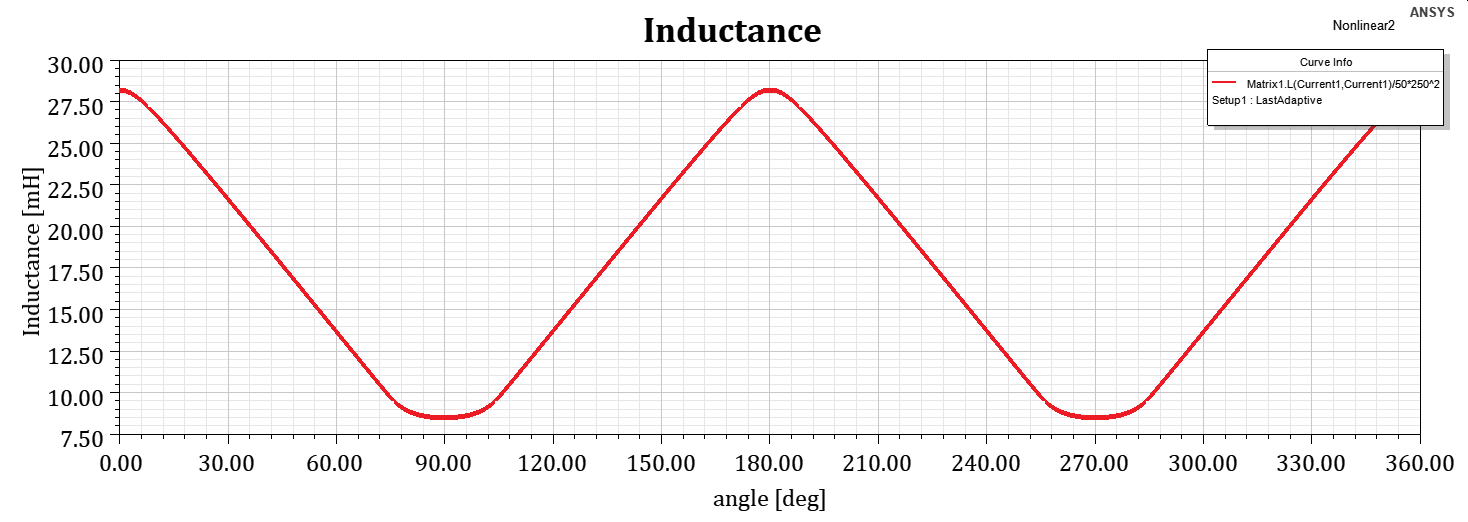
\includegraphics[width=0.75\linewidth]{ind_nonlin_wrtangle.png}
\caption{Inductance of the system assuming non-linear material, as a function of rotor angle}
  \label{fig:ind_nonlin} 
\end{figure}

Torque of the rotor is also obtained for non-linear case, as a function of rotor angle and given in Fig. \ref{fig:torque_angle_nl}. The results are compatible with analytical solution results and are quite similar to the ones obtained in linear material case.\\

\begin{figure}[h!]
\centering
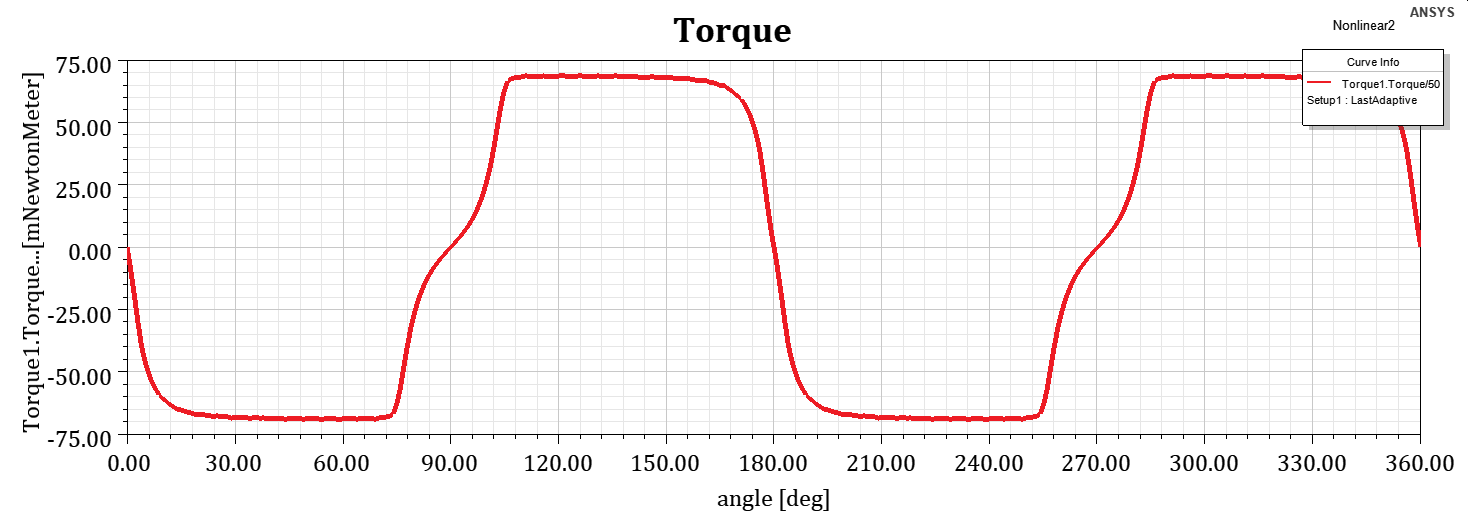
\includegraphics[width=0.75\linewidth]{torque_nonlin_wrtangle.png}
\caption{Torque of the rotor assuming non-linear material, as a function of rotor angle}
\label{fig:torque_angle_nl}
\end{figure}


Magnetic stored energy in the system is obtained using transient analysis. In Fig. \ref{enon1a}, the energy is calculated when $\theta = 0^\circ$, where in Fig. \ref{enon1b}, the energy is calculated for $45^\circ < \theta < 135^\circ$. The minimum energy points are when the rotor is horizontally aligned, and is 38~mJ. Stored energy in the system deviates between 38~mJ and 127~mJ.\\

To observe the effects of linear material assumption, energy calculation is compared with the calculation of $\frac{1}{2}\,L\,I^2$ and co-energy. In Fig. \ref{enon1b}, it can be seen that they differ from each other in non-linear material case.\\

\begin{figure}[h!]
    \centering
  \subfloat[$\theta = 0^\circ$\label{enon1a}]{%
       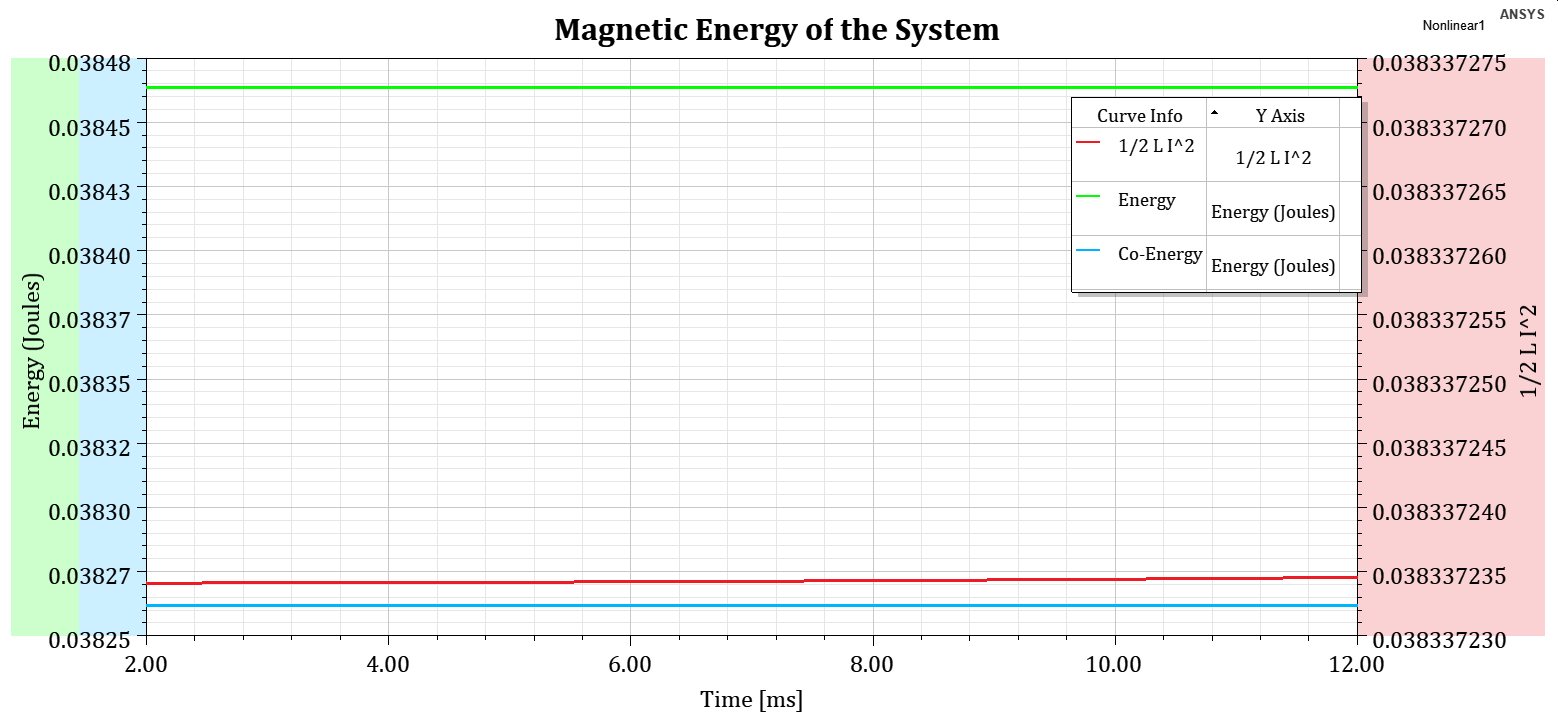
\includegraphics[width=0.45\linewidth]{energy_nlat0deg.png}}
       \hspace{0.5cm}
  \subfloat[$45^\circ < \theta < 135^\circ$\label{enon1b}]{%
        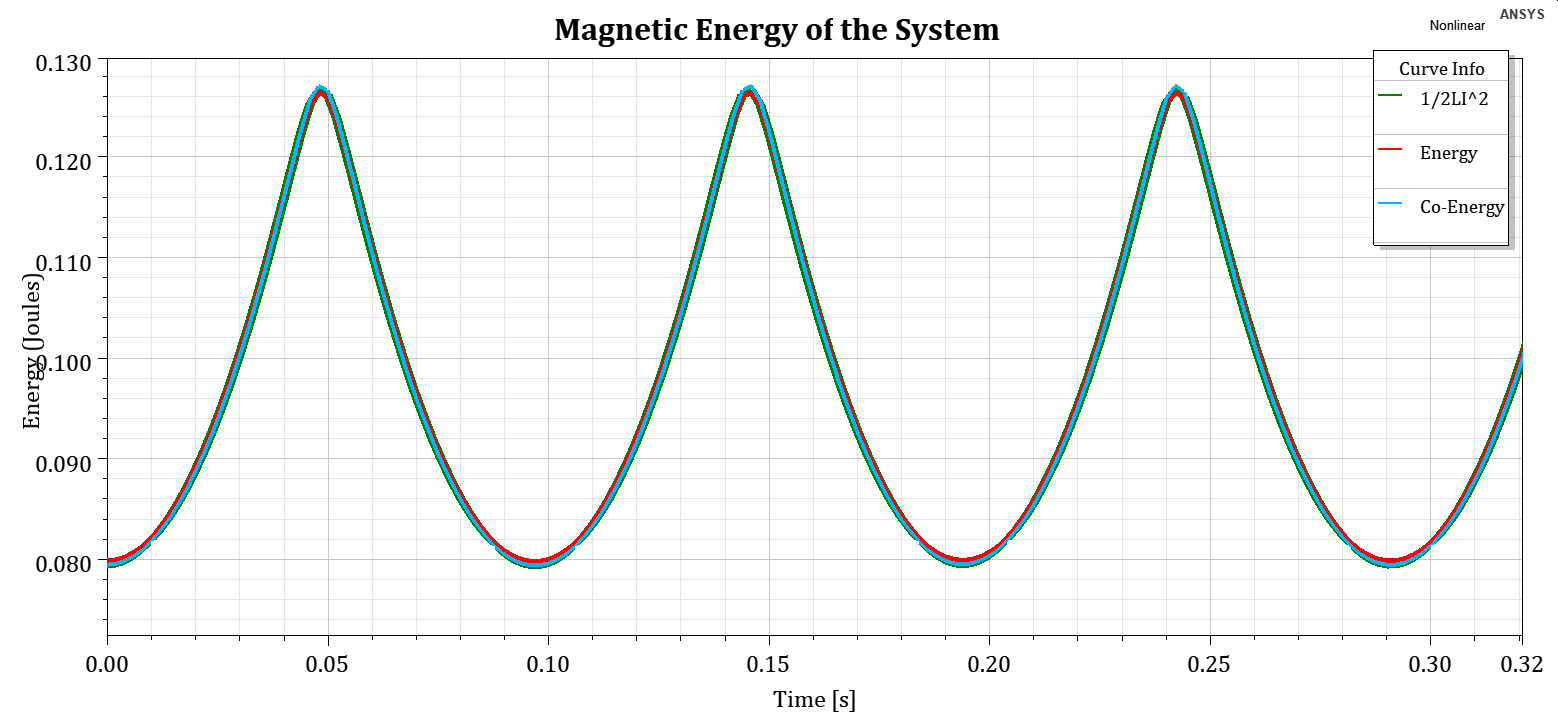
\includegraphics[width=0.45\linewidth]{energy_nl.png}}

  \caption{Magnetic stored energy in the system, assuming non-linear material properties}
  \label{fig:energy_nonlin} 
\end{figure}



\section{Control Method}

In order to accelerate the motor, a positive average torque should be generated. The torque equation is as below:


$$
T(\theta) = \frac{1}{2}\,I^2\,\frac{d\,L(\theta)}{d\theta}
$$

From the equation, it can be figured out that there are two ways to generate positive torque:

\begin{itemize}
\item Apply positive current when the inductance is increasing.
\item Apply negative current when the inductance is decreasing.
\end{itemize}

Similarly, vice versa can be applied to generate negative torque. To keep steady state operation, assuming there is no friction and damping in the system, it is sufficient not to excite the coils.\\

To verify this, the coils are excited with pulse current given in Fig. \ref{fig:pulse}. Resultant torque and speed waveforms of the rotor are given in Fig. \ref{torque1a} and \ref{speed1b}, respectively. Similar approach can be adopted to obtain different torque and speed profiles. \\

\begin{figure}[h!]
\centering
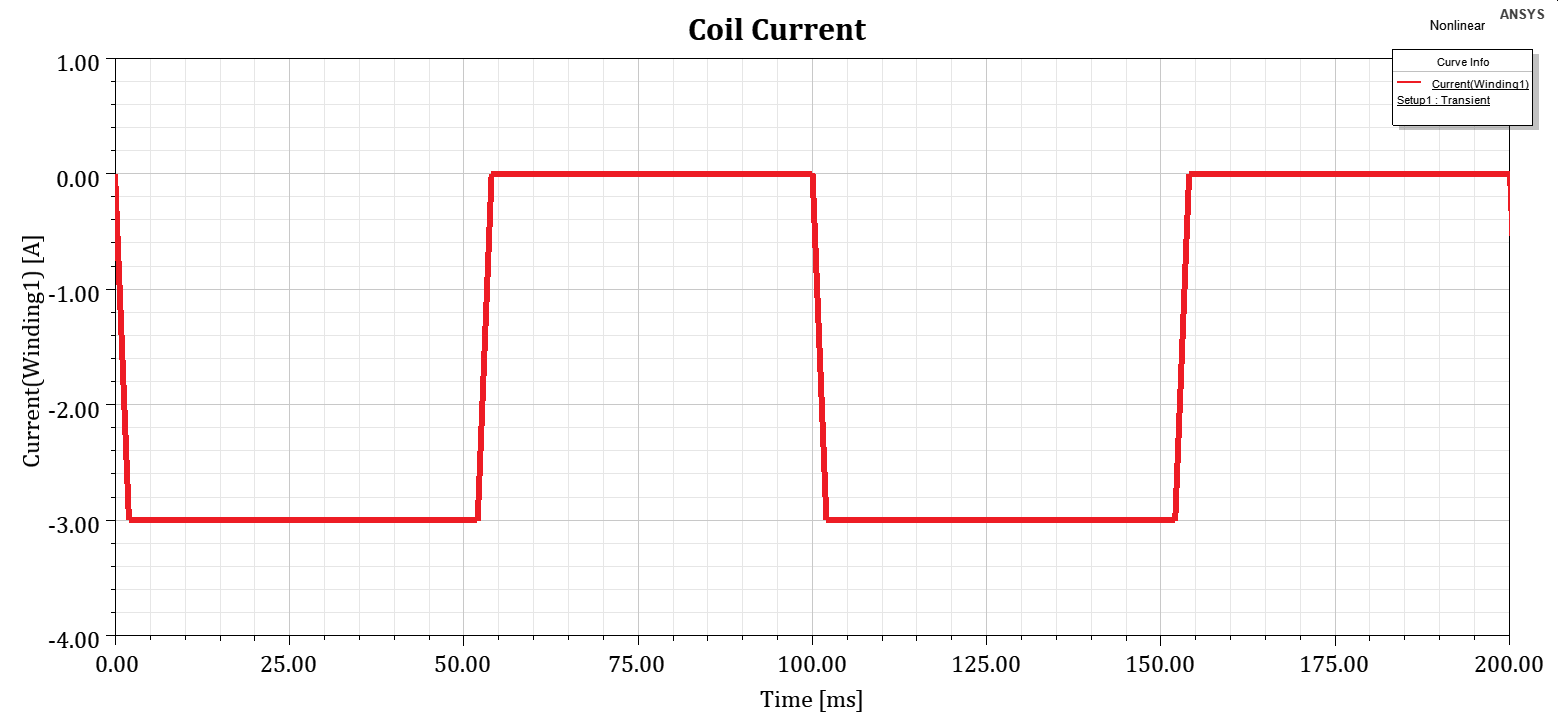
\includegraphics[width=0.75\linewidth]{part4_coil_current.png}
\caption{Pulse current waveform}
\label{fig:pulse}
\end{figure}

\begin{figure}[h!]
    \centering
  \subfloat[Output torque\label{torque1a}]{%
       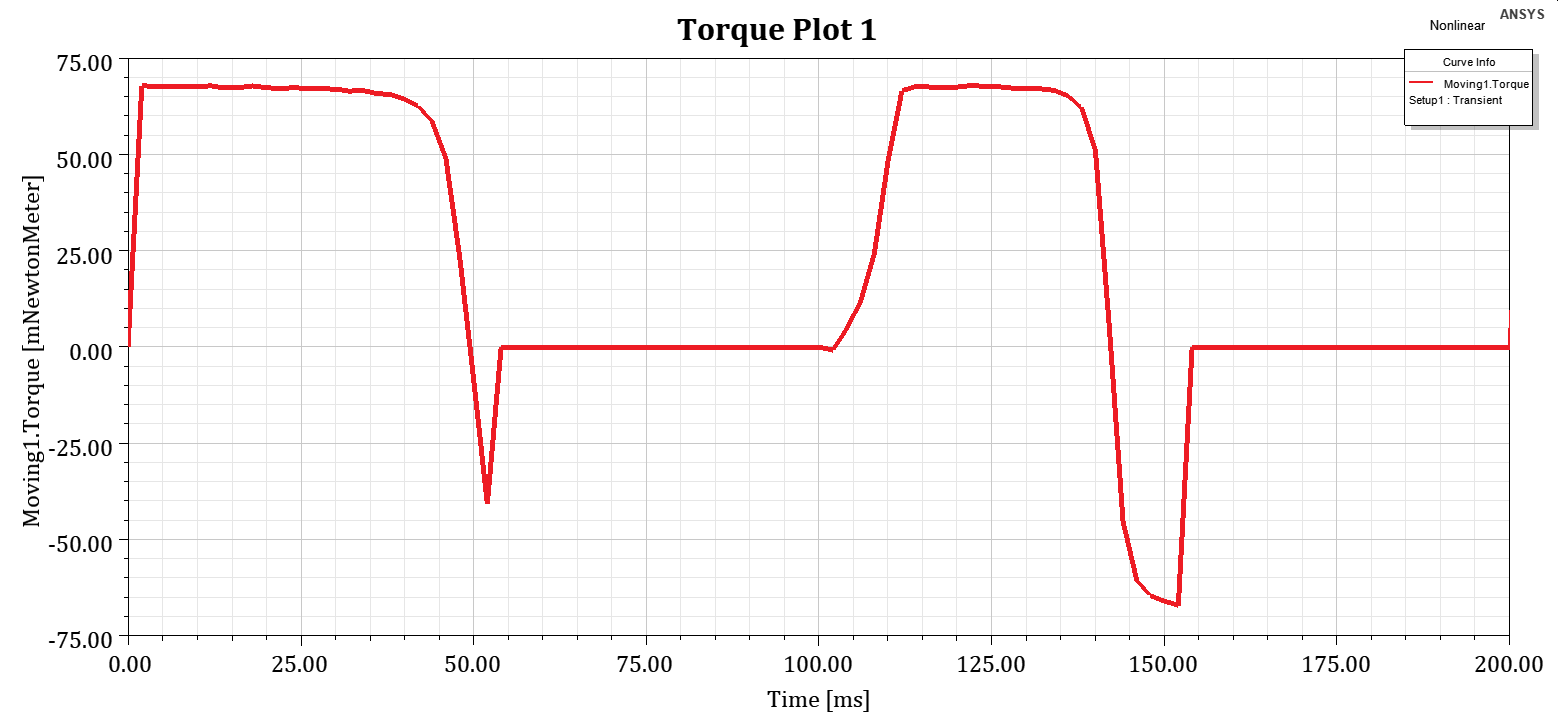
\includegraphics[width=0.45\linewidth]{part4_torque.png}}
       \hspace{0.5cm}
  \subfloat[Rotor speed\label{speed1b}]{%
        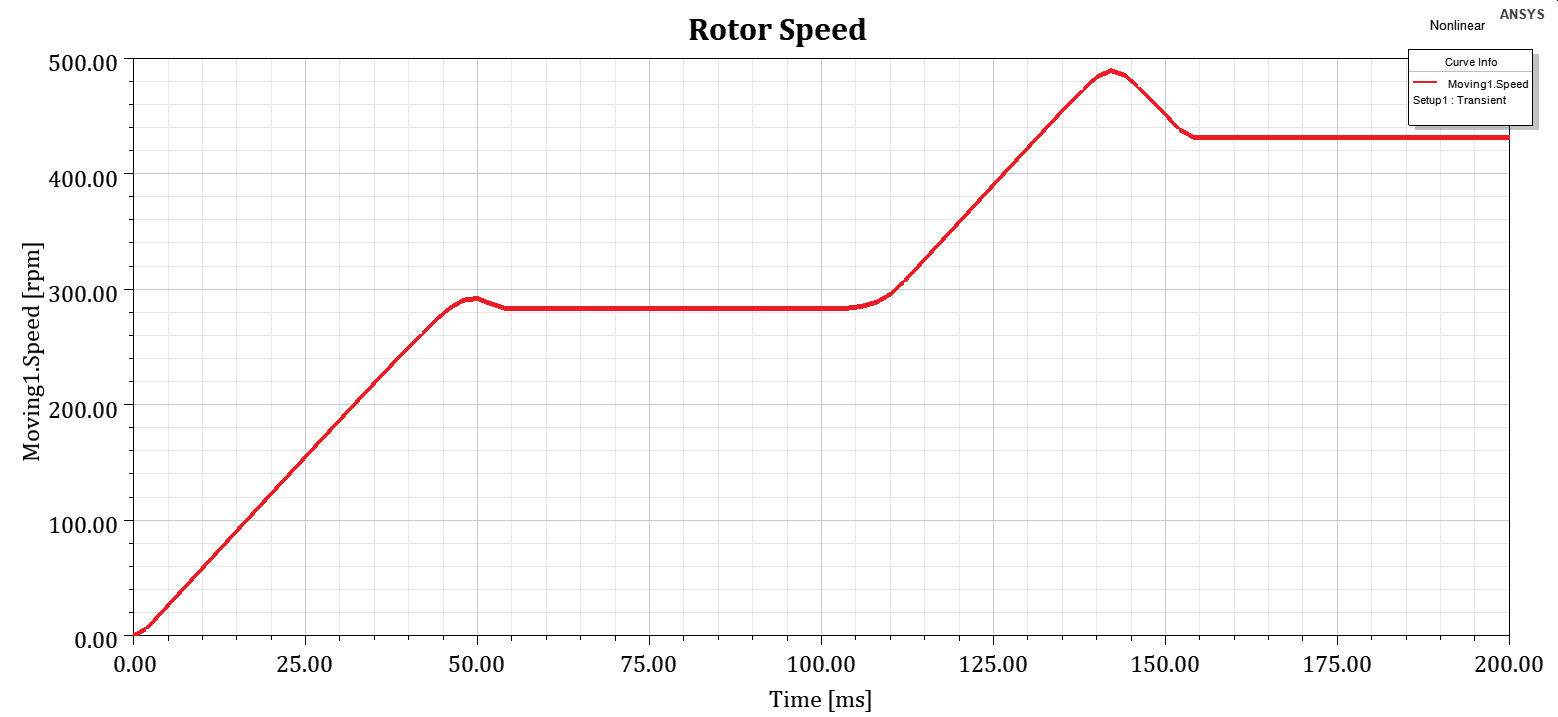
\includegraphics[width=0.45\linewidth]{part4_rotor_speed.png}}

  \caption{Dynamics of the rotor when pulse current is applied}
  \label{fig:energy_nonlin} 
\end{figure}

\section{Animations}

Animations of flux density vectors are obtained in Maxwell 2D environment with transient analysis. They are accessible in the links below:

\begin{itemize}
\item \href{https://github.com/ghandeb/EE568/blob/master/Project%201/kepce.gif}{in this link}.
\item \href{http://www.github.com/ghandeb/EE568}{in this link}.
\item \href{http://www.github.com/ghandeb/EE568}{in this link}.
\end{itemize}

\newpage

\section{Conclusion}

In this project, a simple variable reluctance motor is analyzed using analytical and numerical techniques. Analytical formulations and their results, which are obtained in MATLAB environment, are compared with finite element analysis (FEA) results. The effects and precision of assumptions made for analytical formulations are compared with non-ideal findings. Furthermore, the effects of linear, non-linear material choices, 2D and 3D modelling differences are discussed.


\newpage 

\section*{Appendix: Matlab Code for Analytical Calculations}

    
\subsection*{Analytical Calculations}



\subsubsection*{Initialize}

\begin{verbatim}
close all; clear all; clc;

% Variables and Constants

mu_0 = 4*pi*1e-7;
depth = 20e-3; %m
g1 = 0.5e-3; %m
r0 = 12.5e-3; %m
r1 = 12e-3; %m
g2 = 2.5e-3; %m
r2 = 10e-3; %m
L = 20e-3; %m
N = 250; %turns
I = 3; %Amps
\end{verbatim}
\begin{par}
Reluctance of the system varies over a period. Maximum reluctance position is where the airgap is 2x2.5 mm, i.e. the rotor is in horizontal position. To find the varying reluctance over a period, following angles are defined (see angles.png):
\end{par} \vspace{1em}
\begin{verbatim}
a = asin(7.5/12); %rad
b = asin(7.5/12.5); %rad

alpha = pi/2-(a+b); %rad
\end{verbatim}


\subsubsection*{Reluctance and Inductance Definitions}

\begin{par}
Alpha is the angle where reluctance starts increasing, with respect to flux area, as a function of rotation angle. When rotor angle is alpha, corner of the salient part of the rotor is aligned with the corner of the stator. The change in the reluctance of the straight part of the rotor is ignored.
\end{par} \vspace{1em}
\begin{par}
Reluctance of the system can be defined as a pwl function.
\end{par} \vspace{1em}
\begin{par}
Reluctance for $\theta = 0:\alpha$ and $\theta = 180-\alpha:180$
\end{par} \vspace{1em}
\begin{verbatim}
Rel_min = @(thet) (2*g2)/(mu_0*(2*b-thet)*r0*L);
\end{verbatim}
\begin{par}
Reluctance for $\theta = \alpha:90$
\end{par} \vspace{1em}
\begin{verbatim}
Rel_rise = @(thet) (2*g1)/(mu_0*r1*(thet-alpha)*L);
\end{verbatim}
\begin{par}
Reluctance for $\theta = 90:180-\alpha$
\end{par} \vspace{1em}
\begin{verbatim}
Rel_fall = @(thet) (2*g1)/(mu_0*r1*(pi-alpha-thet)*L);

L_min = @(thet) N^2./Rel_min(thet);

L_rise = @(thet) N^2./(1/Rel_rise(thet)+1/Rel_min(thet-alpha))^(-1);

L_fall = @(thet) N^2./(1/Rel_fall(thet)+1/Rel_min(pi-alpha-thet))^(-1);
\end{verbatim}


\subsubsection*{Plot the Reluctance}

\begin{verbatim}
rot_angle = linspace(0,pi,1000);
Reluctance = zeros(1,length(rot_angle));

for i=1:length(rot_angle)
    t = rot_angle(i);
    if(t<=alpha)
        Reluctance(i) = Rel_min(0);
    end
    if(t>alpha && t<=pi/2)
        Reluctance(i) = Rel_rise(t);
    end
    if (t>pi/2 && t<=(pi-alpha))
        Reluctance(i) = Rel_fall(t);
    end
    if (t>(pi-alpha) && t<=(pi))
        Reluctance(i) = Rel_min(0);
    end

end

rot = linspace(0,2*pi,2000);
Rel_full_rot = [Reluctance,Reluctance];


figure;
plot(rot,Rel_full_rot,'LineWidth',2);
grid minor;
xlabel('Rotation Angle (rad)','FontSize',16);
ylabel('Reluctance (1/H)','FontSize',16);
ylim([0 5e7]);
title('Reluctance of the System','FontSize',16);
saveas(gcf,'Reluctance_analytical','epsc');
\end{verbatim}
\begin{center}
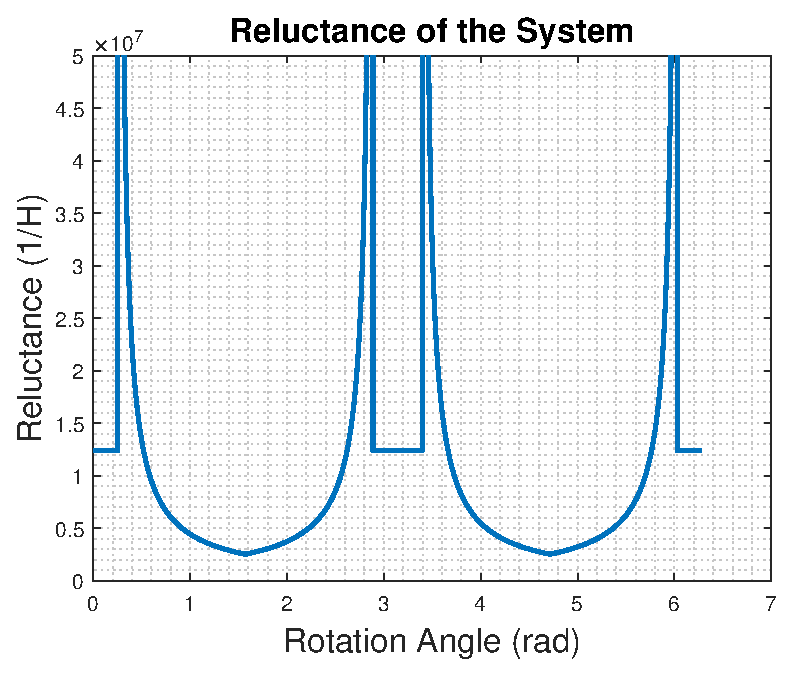
\includegraphics[width=4in]{html/analytical_01.eps}
\end{center}



\subsubsection*{Plot the Inductance}

\begin{verbatim}
rot_angle = linspace(0,pi,1000);
Inductance = zeros(1,length(rot_angle));

for i=1:length(rot_angle)
    t = rot_angle(i);
    if(t<=alpha)
        Inductance(i) = L_min(0);
    end
    if(t>alpha && t<=pi/2)
        Inductance(i) = L_rise(t);
    end
    if (t>pi/2 && t<=(pi-alpha))
        Inductance(i) = L_fall(t);
    end
    if (t>(pi-alpha) && t<=(pi))
        Inductance(i) = L_min(0);
    end

end

rot = linspace(0,2*pi,2000);
Ind_full_rot = [Inductance,Inductance];


figure;
plot(rot,Ind_full_rot,'LineWidth',2);
grid minor;
xlabel('Rotation Angle (rad)','FontSize',16);
ylabel('Inductance (H)','FontSize',16);
ylim([0 0.03]);
title('Inductance of the System','FontSize',16);
saveas(gcf,'inductance_analytical','epsc');
\end{verbatim}

\begin{center}

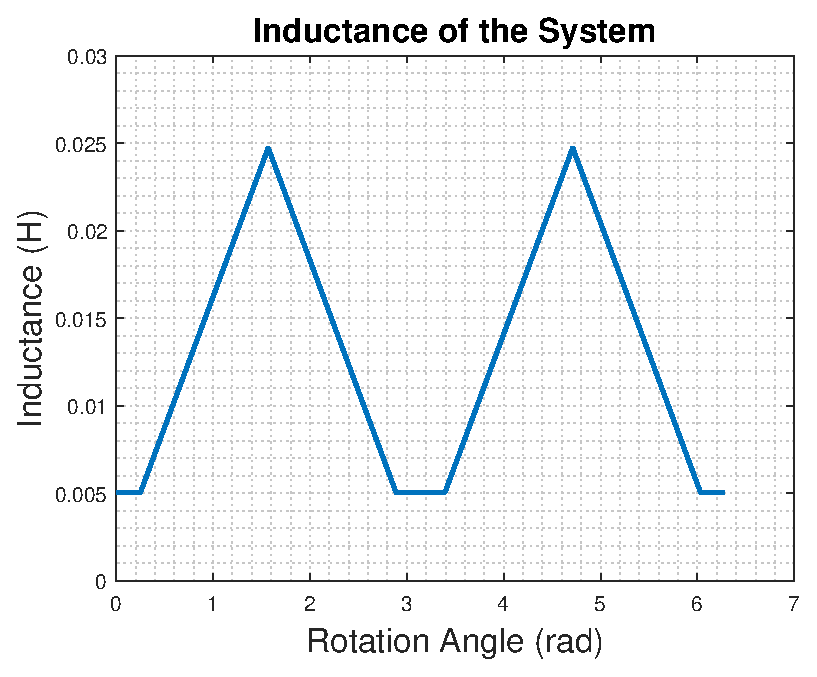
\includegraphics [width=4in]{html/analytical_02.eps}

\end{center}

\subsubsection*{Torque Calculation}

\begin{par}
$T = \frac{1}{2}\cdot I^2\cdot\frac{dL(\theta)}{d\theta}$
\end{par} \vspace{1em}
\begin{verbatim}
Torque_full_rot = zeros(size(Ind_full_rot));

for i = 1:length(Torque_full_rot)-1
    Torque_full_rot(i+1) = (Ind_full_rot(i+1)-Ind_full_rot(i))/(rot(i+1)-rot(i));
end

Torque_full_rot = Torque_full_rot*I^2/2;

figure;
plot(rot,Torque_full_rot,'LineWidth',2);
grid minor;
xlabel('Rotation Angle (rad)','FontSize',16);
ylabel('Torque (Nm)','FontSize',16);
% ylim([0 0.03]);
title('Torque of the Rotor','FontSize',16);
saveas(gcf,'torque_analytical','epsc');
\end{verbatim}

\begin{center}

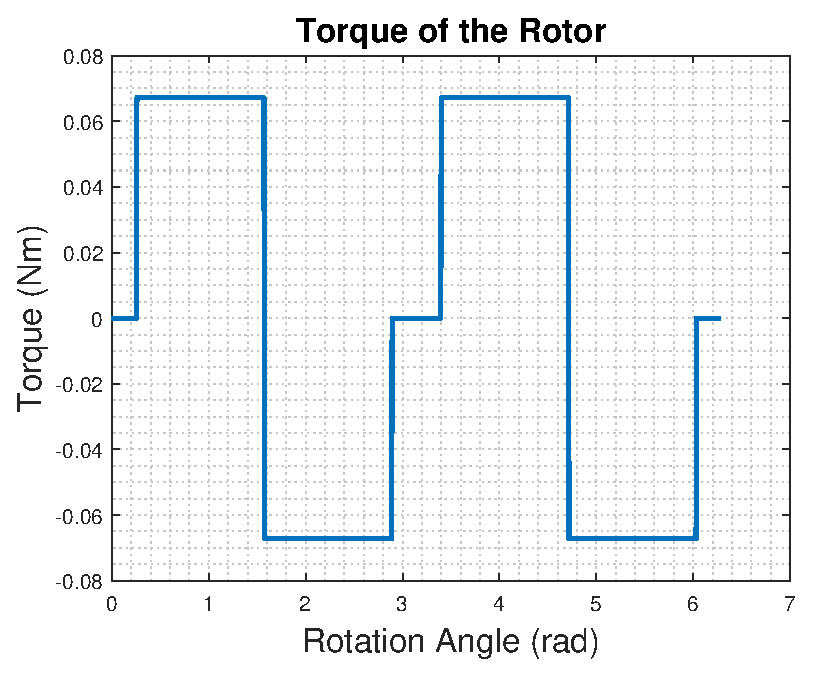
\includegraphics [width=4in]{html/analytical_03.eps}

\end{center}




\end{document}
